%%%%%%%%%%%%%%%%%%%%%%%%%%%%%%%%%%%%%%%%%%%%%%%%%%%%%%%%%%%%%%%%%%%%%%%%%%%%%%%

\chapter{ANÁLISE E RESULTADOS}
\label{capanaliseseresults}

A possível natureza caótica da turbulência na camada limite atmosférica, no interior e acima da copa da floresta é investigada. Com base na aplicação de diversas ferramentas
%(já descritas no Capítulo~\ref{caputiltecnicas}) 
nas séries temporais em estudo, o objetivo deste trabalho é determinar se tais séries incluem componentes determinísticas que podem ser descritas (individualmente) por um sistema dinâmico de baixa dimensão, que se desenvolve em um atrator caótico.


\section{Estacionaridade}
Primeiramente, as séries temporais em estudo foram submetidas ao teste de estacionaridade.
% já descrito na Seção~\ref{subsecestacio}. 
A Tabela~\ref{tabelatempestacionaria} apresenta a classificação destas séries em estacionárias ou não estacionárias. Neste teste foram utilizadas janelas de dados deslizantes variáveis, a saber, $L=100,500$ e $1000$. Desta forma, as análises subseqüentes serão feitas apenas com as séries do tipo estacionárias.

\begin{table}[!ht]
\begin{center}
\caption{Análise da estacionaridade para as séries temporais de temperatura e velocidade do vento em diferentes períodos do dia e níveis da copa.}
\begin{tabular}{c c c}
\hline 
\textbf{Série temporal} & \textbf{Estacionaridade} \\
\hline
tS1200 & estacionária \\
tI1200 & estacionária \\
tS2300 & não-estacionária \\
tI2300 & estacionária \\
tM1200 & estacionária \\
wS1200 & estacionária \\
tM2300 & não-estacionária \\
\hline
\end{tabular}
\label{tabelatempestacionaria}
\end{center}
\end{table}

\section{Decomposição dos Dados}

Com o objetivo de investigar o papel das estruturas coerentes na existência (ou não) de caos na atmosfera, decidiu-se selecionar dentre o conjunto de séries disponíveis uma que apresentasse sinais nítidos da presença de estruturas coerentes em rampa e em seguida decompor a mesma (denominada de série total) em duas partes: uma parte dita coerente (baixas freqüências) e uma parte incoerente (altas freqüências). A parte coerente é caracterizada apenas pelas estruturas coerentes em rampa presentes na série total, enquanto que a parte incoerente é caracterizada pelas flutuações aparentemente aleatórias da mesma série. 

%\subsection{Decomposição dos dados}

Inicialmente, a série temporal total (tS1200) foi decomposta em suas partes coerente e incoerente, por meio da filtragem com Wavelet de Haar~\cite{katul/94}, que é um tipo de ondeleta-mãe discreta, definida por

\begin{equation}
\left\{ \begin{array}{rrr} 1, &  & 0\leq t < 1/2 \\
                  -1, &  & 1/2\leq t < 1 \\
		   0, &  & \mbox{caso contrário}
\end{array} 
\right.
\label{eqwavelethaar}
\end{equation} 

Esta categoria de ondaletas é utilizada para detectar variações bruscas nos sinais, e trabalha com sinais temporais que tenham comprimentos da ordem da potência de dois mais próxima, ou seja, $2^{f}=s$, onde $s$ é o comprimento total da série, e $f$ é o número de freqüências possíveis para a decomposição. 

O comprimento da série em estudo é de $s=108.000$ pontos. Desta forma, não há um número exato de decomposições em freqüências, já que $f=16$ resulta em $s=65.536$ pontos e $f=17$ resulta em $s=131.072$ pontos. A estratégia utilizada foi completar o início da série temporal com zeros até que a freqüência $f=17$ fosse alcançada. 
 
Ainda não há na literatura um consenso de qual seja a melhor função ondeleta a ser utilizada para a decomposição e filtragem de uma série temporal. O que comumente se aceita é que a função ondeleta possua um formato característico próximo das características encontradas na série temporal. Isso explica o fato da Wavelet de Haar ter sido escolhida para a decomposição da série temporal de temperatura.  

A Figura~\ref{figfiltrotS0681200} mostra a série temporal total, a série temporal coerente (soma das baixas freqüências da série total) e a série temporal incoerente (soma das altas freqüências da série total), respectivamente. Após a filtragem da série total, $23072$ pontos iniciais foram descartados das séries total, coerente e incoerente; tal valor corresponde ao número de zeros inseridos na série total antes do procedimento de filtragem. É importante ressaltar que a soma da série coerente com a série incoerente resulta a série total, o que já era esperado.

\begin{figure}[ht]
	\caption{Séries temporal total, coerente e incoerente.}
	\vspace{0mm}	% acrescentar o espaçamento vertical apropriado entre o título e a borda superior da figura
	\begin{center}
		\resizebox{13cm}{!}{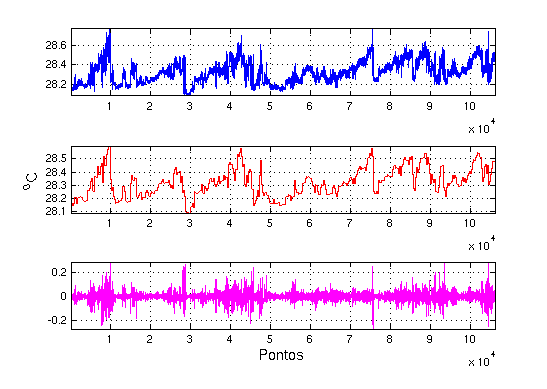
\includegraphics{Figuras2/filtrocoltS0681200.png}}		
	\end{center}
	\vspace{-2mm}	% acrescentar o espaçamento vertical apropriado entre a borda inferior da figura e a legenda ou a fonte quando não há legenda (o valor pode ser negativo para subir)
	\legenda{Sinal total (superior), soma das nove primeiras freqüências (meio), soma das sete últimas freqüências (inferior).}	% legenda - para deixar sem legenda usar comando \legenda{} (nunca deve-se comentar o comando \legenda)
	\label{figfiltrotS0681200}
	\FONTE{Produção do autor.}	% fonte consultada (elemento obrigatório, mesmo que seja produção do próprio autor)
\end{figure}

\section{Caracterizando a turbulência acima da copa da floresta Amazônica}

O objetivo desta seção é verificar se as séries total, coerente e incoerente possuem as características típicas da turbulência plenamente desenvolvida, a saber, espectros de potência do tipo Kolmogorov e intermitência nas pequenas escalas. Aproveita-se para ilustrar o papel crucial das estruturas coerentes no transporte de propriedades (quantidade de movimento, calor, etc.) através da copa da floresta.

\subsection{Espectros de potência}

Os espectros de potência das séries temporais total, coerente e incoerente foram estimados usando FFT (ver Figura~\ref{figespectrotS0681200}). Os resultados mostram que as inclinações desses espectros no SI (em escala $\log$-$\log$) coincidem com a lei dos $-5/3$ de Kolmogorov. Esta observação demonstra que o fenômeno da turbulência está presente na série total, o que era esperado, mas também nas séries coerente e incoerente. Em especial, pode-se afirmar que a série incoerente está mais relacionada à turbulência de pequena escala do que a algum tipo de ruído. Este comportamento é consistente com outros estudos que utilizaram a mesma abordagem de separação de um fluxo turbulento em uma parte coerente e outra incoerente~\cite{farge/01}.

\begin{figure}[ht]
	\caption{Espectros de potência das séries temporais total, coerente e incoerente.}
	\vspace{0mm}	% acrescentar o espaçamento vertical apropriado entre o título e a borda superior da figura
	\begin{center}
		\resizebox{15cm}{!}{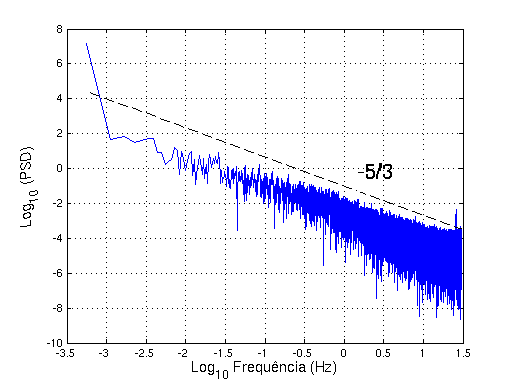
\includegraphics{Figuras2/tS0681200espectro.png}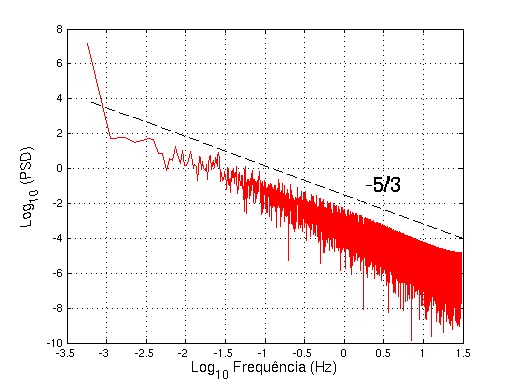
\includegraphics{Figuras2/ctS0681200espectro.png}}\\ \resizebox{7.5cm}{!}{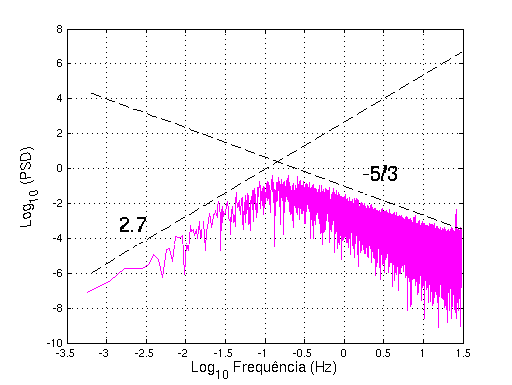
\includegraphics{Figuras2/itS0681200espectro.png}}		
	\end{center}
	\vspace{2mm}	% acrescentar o espaçamento vertical apropriado entre a borda inferior da figura e a legenda ou a fonte quando não há legenda (o valor pode ser negativo para subir)
	\legenda{Em azul espectro de potência da série temporal total, em vermelho da série temporal coerente e em rosa da série temporal incoerente. Observe que as inclinações de todos os espectros no SI (em escala $\log$-$\log$) coincidem com a lei dos $-5/3$ de Kolmogorov. O espectro de potência associado a série incoerente possui uma inclinação adicional de $2.7$, que pode estar associada a um artefato numérico.}	% legenda - para deixar sem legenda usar comando \legenda{} (nunca deve-se comentar o comando \legenda)
	\label{figespectrotS0681200}
	\FONTE{Produção do autor.}	% fonte consultada (elemento obrigatório, mesmo que seja produção do próprio autor)
\end{figure}

\subsection{Intermitência}

A detecção do fenômeno intermitente foi feita a partir das diferenças das séries de temperatura total, coerente e incoerente (medida às $12$ horas no nível superior) em várias escalas $r_{i}$ com $i=1,\ldots4$. Desta forma, as FDP's foram obtidas com base na distribuição estatística das diferenças $\Delta T_{r_{i}}=T(x+\Delta r_{i})-T(x)$. Os valores assumidos por $\Delta r_{i}$ são dados respectivamente por $1,10,100$ e $1000$, que para dados amostrados à $60$ Hz correspondem a $\Delta T_{t_{i}}$ de aproximadamente $0.0167,0.1667,1.6667$ e $16.6667$ segundos, respectivamente.